% Chapter Template

\chapter{Results} % Main chapter title

\label{Chapter4} % Change X to a consecutive number; for referencing this chapter elsewhere, use \ref{ChapterX}

%----------------------------------------------------------------------------------------
%	SECTION 1
%----------------------------------------------------------------------------------------
\section{Qualitative and quantitive descriptions of slow waves}
After slow oscillations in the df/f signal were detected an event related analysis was performed and individual waves were investigated qualitatively. Waves with a peak amplitude below 5\% were excluded from the main analysis. 

\begin{figure}[!htb]
\centering
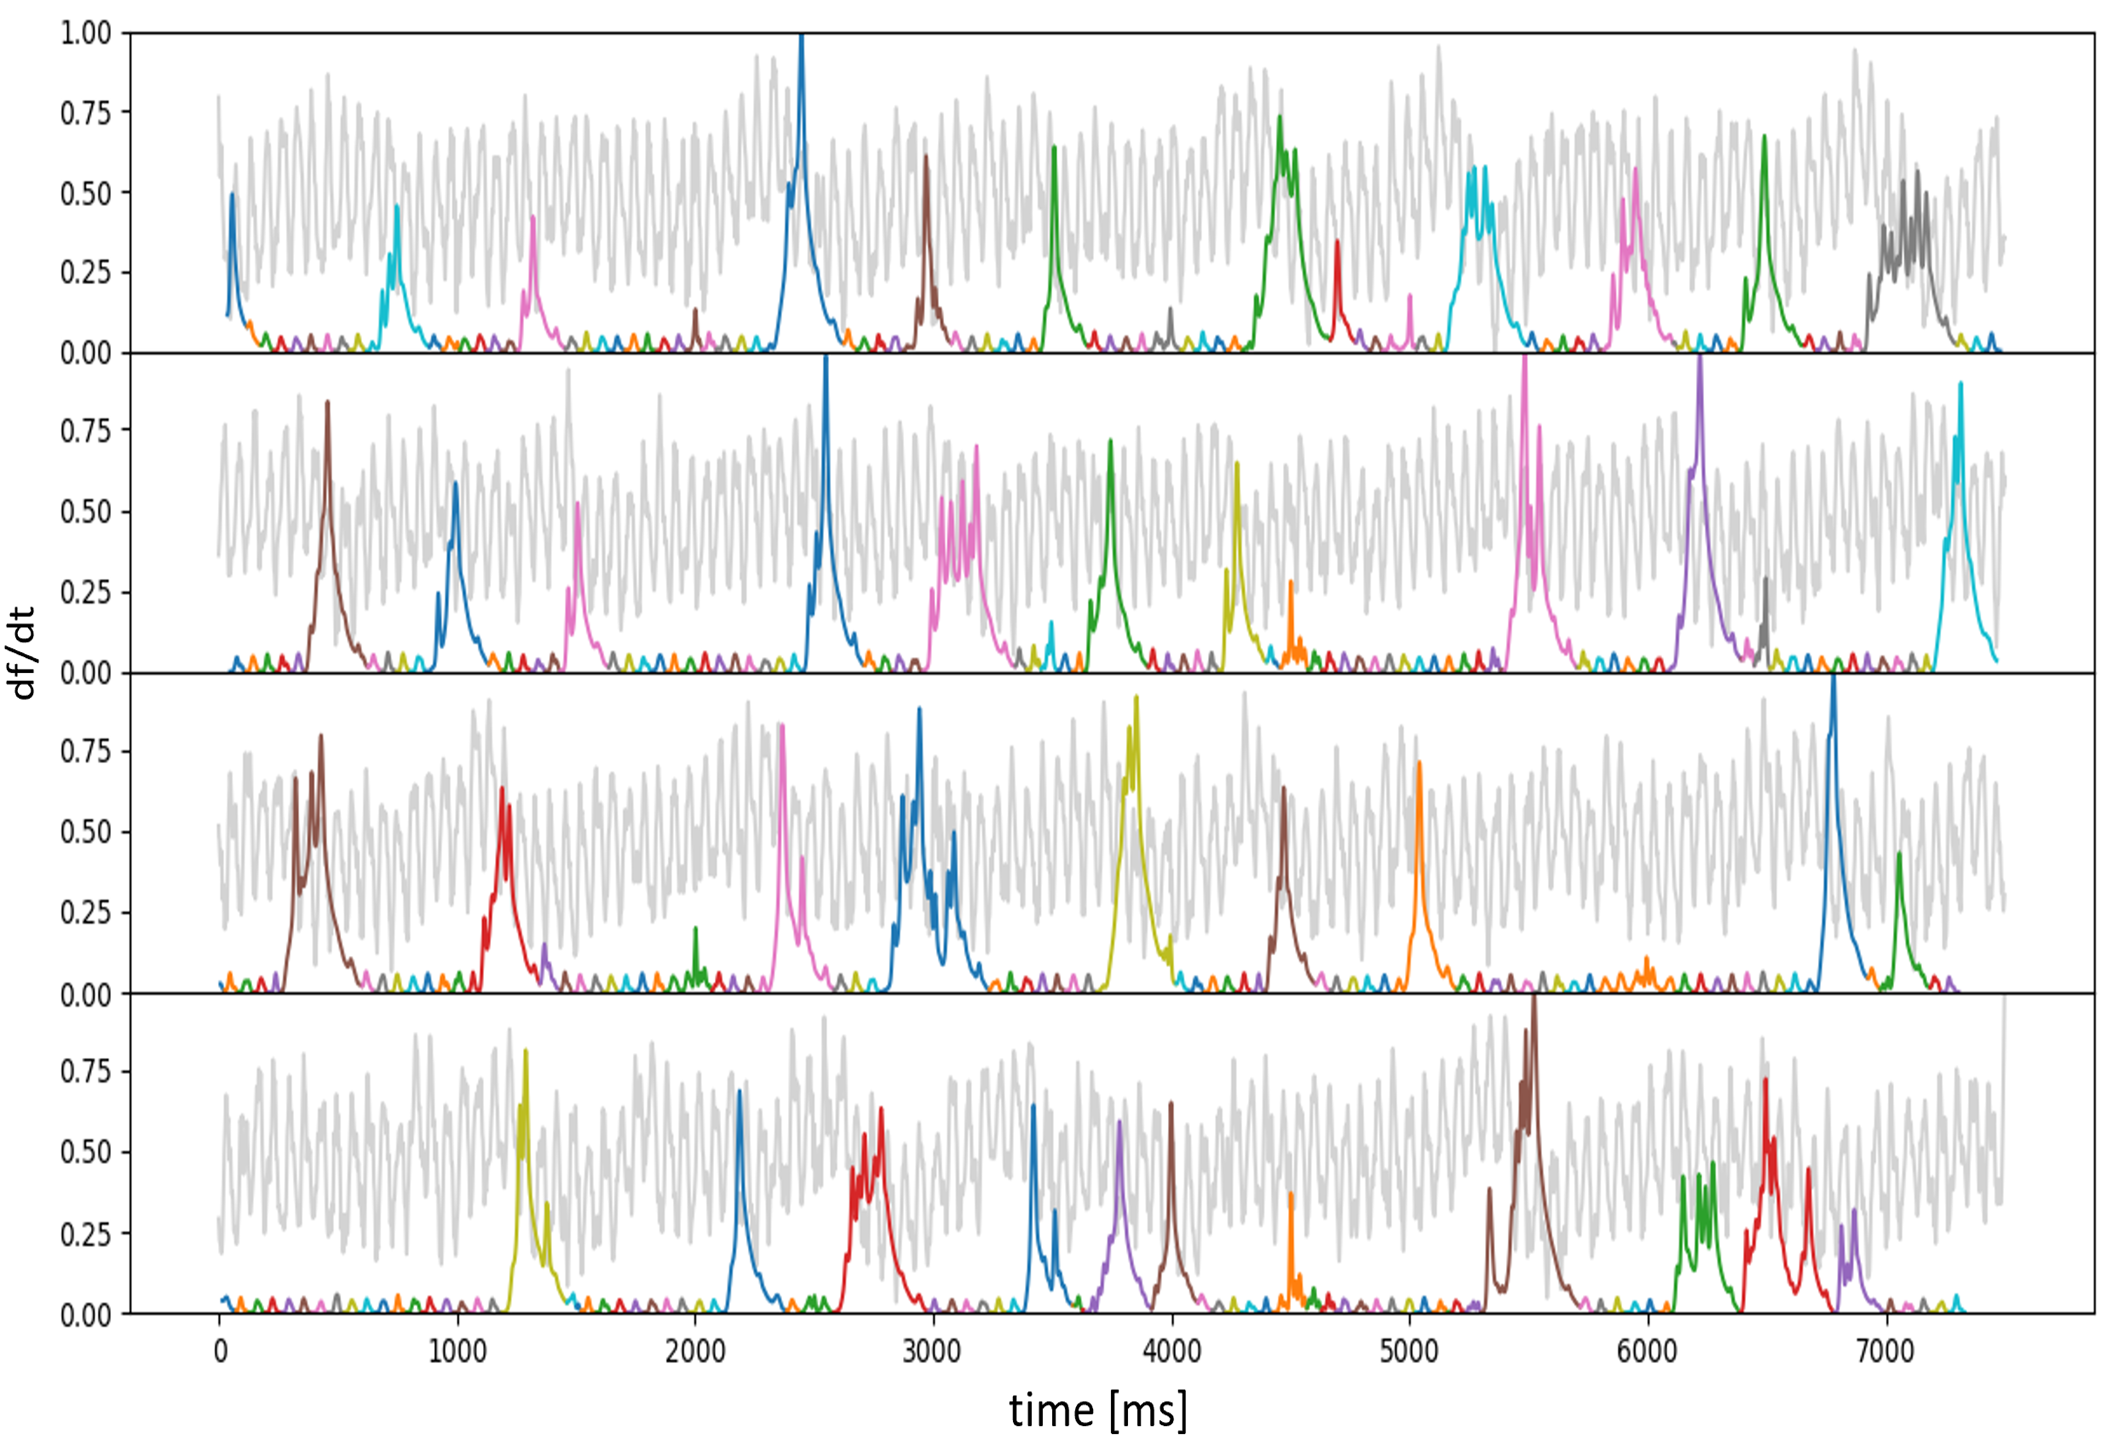
\includegraphics[width=\textwidth,height=\textheight,keepaspectratio]{Figures/slow_wave_segmentation}
\decoRule
\caption[Detected slow waves for a sample recording]{Detected slow waves for a sample recording at 1.8 \% isoflurane.\\ The depiction shows the results of the splitting procedure. Segments of the baseline-corrected mean percentage change that were identified as one event are represented in the same color. Note that the approach identifies events in a scale independent manner. The depiction shows the mean percentage change for a complete recording at 1.8 \% isoflurane. Note also that several events are similar with respect to shape and size. Different types can be distinguished.}
\label{fig:slow_wave_segmentation}
\end{figure}

\begin{figure}[!htb]
\centering
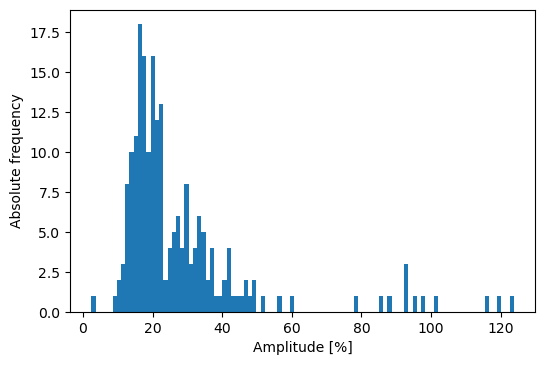
\includegraphics[width=\textwidth,height=\textheight,keepaspectratio]{Figures/selected_waves_distribution_of_peak_amplitude}
\decoRule
\caption[Distribution of the peak amplitude of detected waves]{Distribution of the peak amplitude of detected waves.\\The depiction shows the distribution of the peak amplitude of the selected slow waves after cleaning the dataset. Cleaning includes removal of instances that are highly correlated (r>.3) with the hemodynamic breathing signal. In addition, it comprises the removal of waves for which the peak activity of the mean percentage change in time is less than 5\% of the duration. Note that events with a peak amplitude of below 5\% are almost completely absent.}
\label{fig:selected_waves_distribution_of_peak_amplitude}
\end{figure}

\begin{figure}[!htb]
\centering
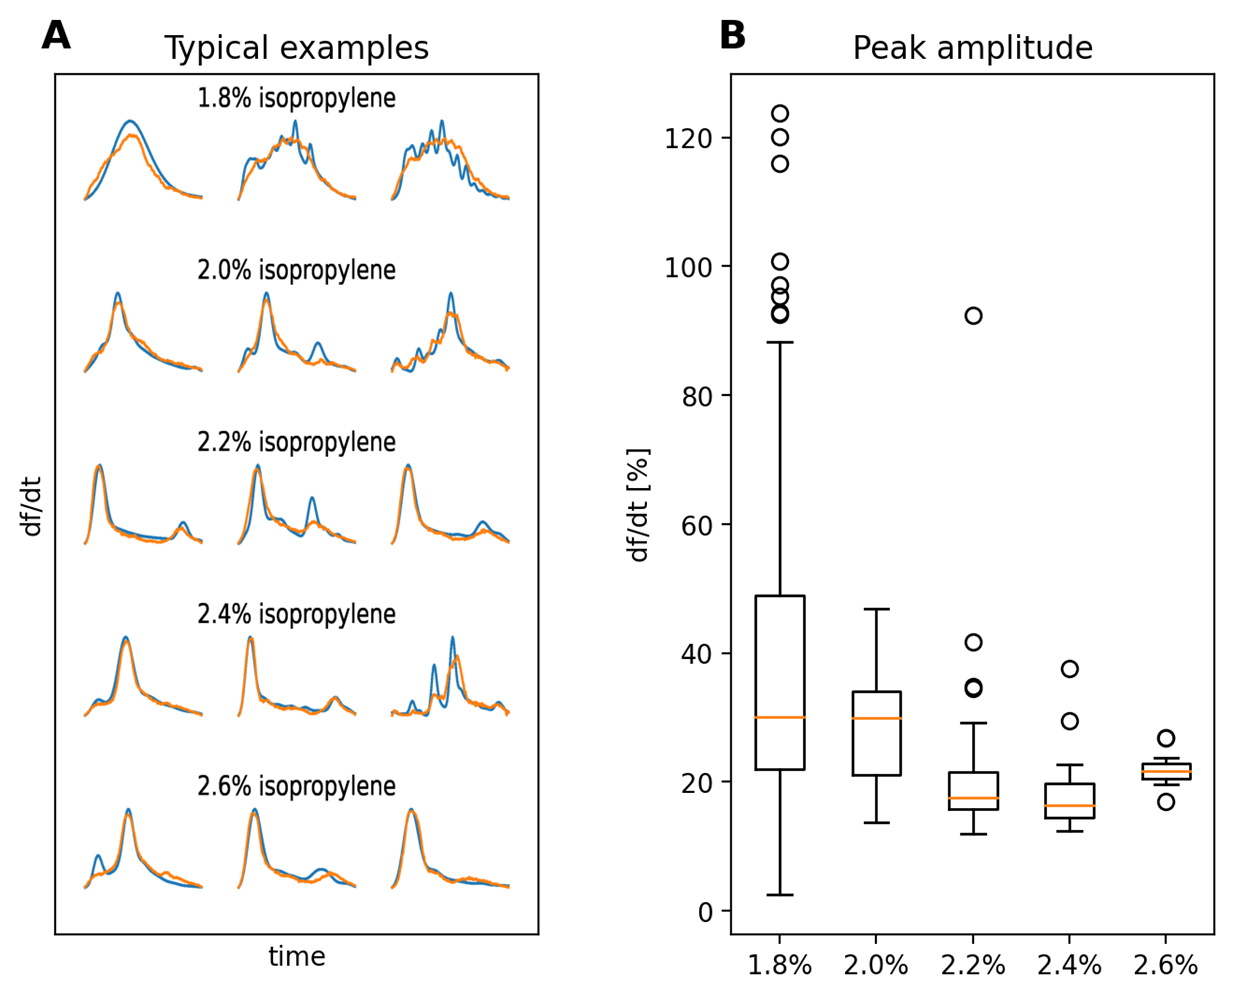
\includegraphics[width=\textwidth,height=\textheight,keepaspectratio]{Figures/typical_examples_and_peak_amplitudes}
\decoRule
\caption[Typical examples and peak amplitudes]{Typical examples and peak amplitudes.\\The depiction shows data for slow waves with a peak amplitude above 5\% that are only weakly correlated with the hemodynamic signal (r < .3). Panel A: Typical examples for slow-wave events during different stages of anesthesia. The mean signal change over time is indicated in blue while reconstructions of the Variational Autoencoder with fully connected layers are plotted in orange. Panel B: The distribution of the peak amplitudes of the mean signal over time for each slow wave per condition.}
\label{fig:typical_examples_and_peak_amplitudes}
\end{figure}

\begin{figure}[!htb]
\centering
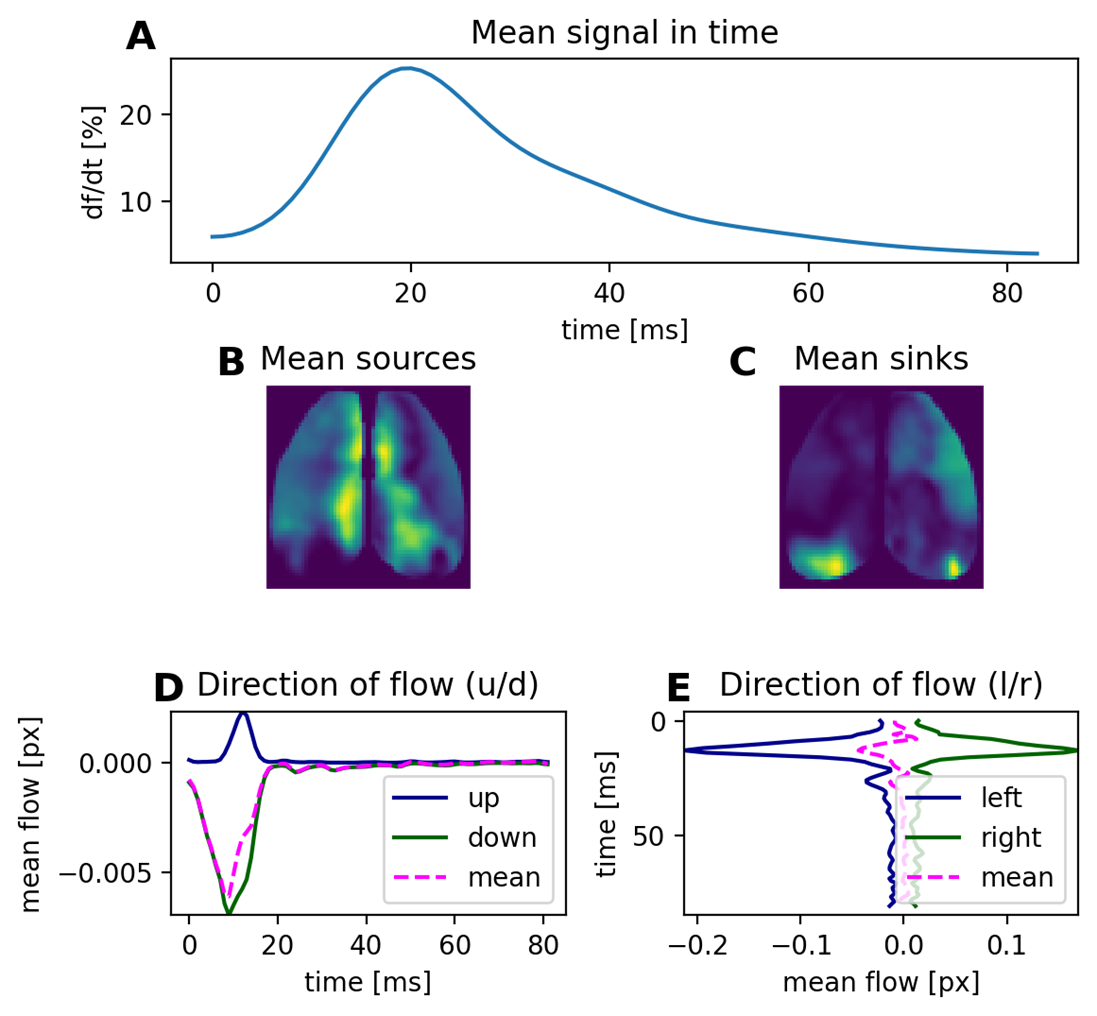
\includegraphics[width=\textwidth,height=\textheight,keepaspectratio]{Figures/percentage_change_direction_of_flow_and_sources_sinks}
\decoRule
\caption[A typical example with one peak]{A typical example with one peak.\\Percentage change, direction of flow and the distribution of sources and sinks. Panel A shows the mean percentage change in time. Panel B illustrates the mean sources and sinks distribution in space and Panel C illustrates the mean sinks distribution respectively. Note that the brain regions that act as sources are not identical with the regions that act as sinks which supports the idea of a sender-receiver pattern. Panels D and E indicate the direction of flow in vertical direction (up/down) and horizontal direction (leftwards/rightwards) respectively.}
\label{fig:percentage_change_direction_of_flow_and_sources_sinks}
\end{figure}


\begin{figure}[!htb]
\centering
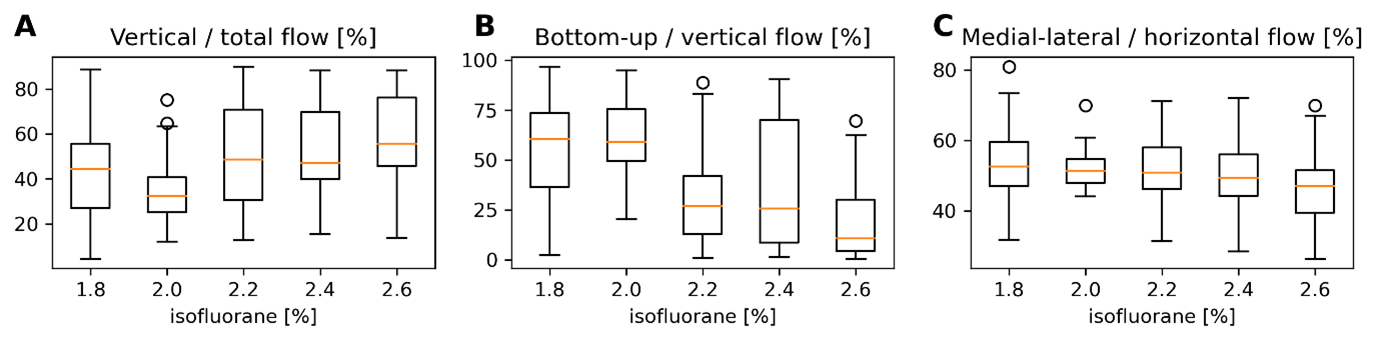
\includegraphics[width=\textwidth,height=\textheight,keepaspectratio]{Figures/direction_per_isoflourane}
\decoRule
\caption[Direction of flow for different levels of isoflurane]{The direction of flow for different levels of isoflurane.\\Panel A: Vertical flow (the sum of the absolute Y-components of the vectors of the flow field) as a proportion of total flow. Panel B: Bottom-up flow as a proportion of vertical flow. Panel C: Medial to lateral flow as a proportion of horizontal flow (the sum of absolute X-components of the vectors of the flow field). Note that the flow component retrieved via Helmholtz-Decomposition of the Optical-Flow are the basis for the aggregated data displayed here.}
\label{fig:direction_per_isoflourane}
\end{figure}

\begin{figure}[!htb]
\centering
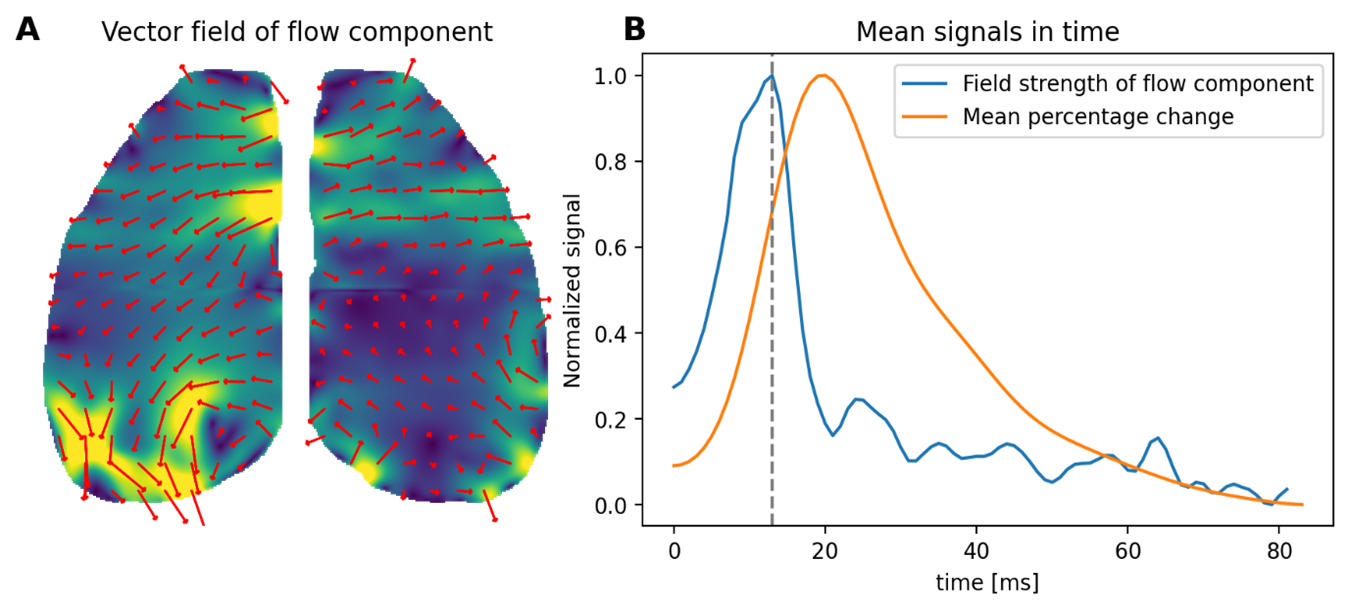
\includegraphics[width=\textwidth,height=\textheight,keepaspectratio]{Figures/vector_field_flow_component}
\decoRule
\caption[A sample vector field and field strength of flow in time.]{A sample vector field and field strength of flow in time.\\ The depiction shows a vector field for a slow-wave event at 1.8\% isoflurane alongside the mean percentage change and mean flow in time. Panel A: The vector field representation of the flow component. The field strength is plotted in the background. Panel B: The mean percentage change in time and the mean field strength of the flow component. Note that the signals are not to scale. The time of the depicted frame is marked by a vertical dotted line. Left-downwards flow shows for the left hemisphere.}
\label{fig:vector_field_flow_component}
\end{figure}

\begin{figure}[!htb]
\centering
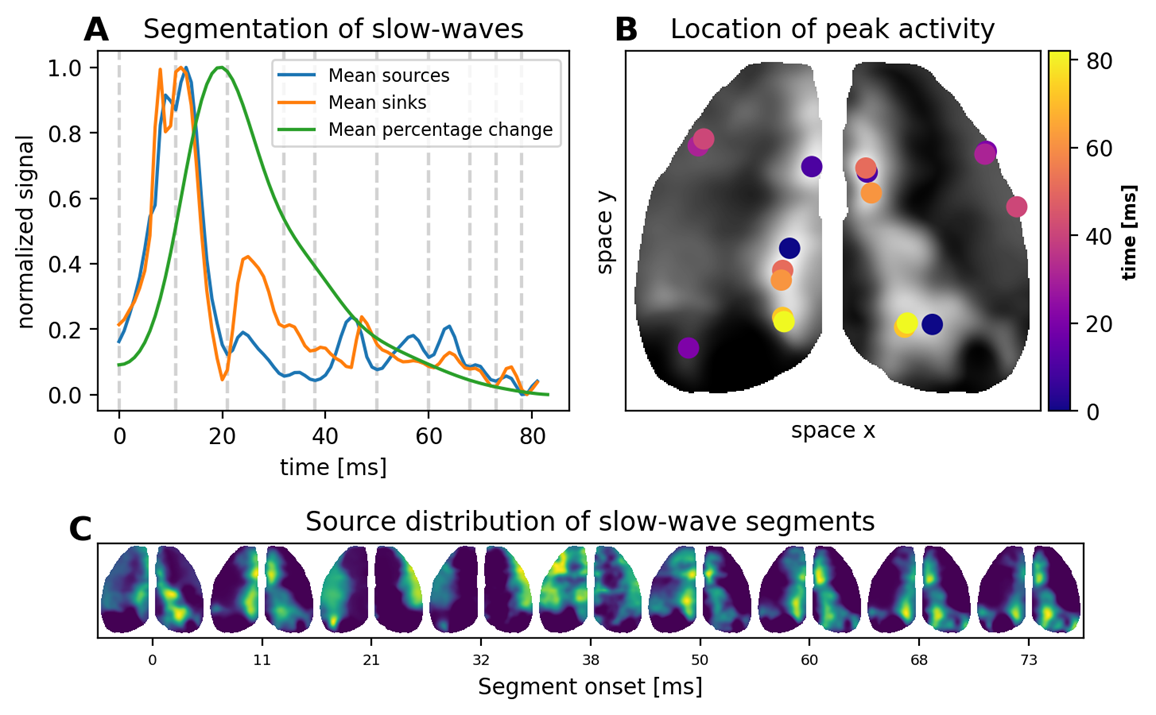
\includegraphics[width=\textwidth,height=\textheight,keepaspectratio]{Figures/slow_wave_subsegements}
\decoRule
\caption[Slow wave subsegments]{Slow wave subsegments.\\The depiction illustrates the procedure of splitting a slow wave into subsegments using the mean sources distribution. Panel A: The mean signal in time for the sources and sinks alongside the mean percentage change. Slow-wave segments are determined using local minima in the mean sources signal in time. Gray dotted lines indicate the onset and offset of each segment. Panel B: The location of peak activity. Panel B shows the location of maximal activity for the mean source signal in space of each subsegment (see Panel C). Note that the time of segment-onset is indicated by different colours. Each dot corresponds to the segments identified in A and the mean source signal in space in C. Panel C: The mean source signal in space for the identified slow-wave segments. During different stages of the slow-wave different areas act as sources. They can coarsely be distinguished into a lateral cluster including somatosensory areas (e.g. segment onset at 21ms) and a medial cluster that includes regions on the medial axis from frontal to occipital cortex.}
\label{fig:slow_wave_subsegements}
\end{figure}

\begin{figure}[!htb]
\centering
\includegraphics[width=\textwidth,height=\textheight,keepaspectratio]{Figures/sources_are_not_mean_signal}
\decoRule
\caption[Sources are not the mean signal]{Sources are not the mean signal\\ The depiction illustrates that the average of all frames showing the df/f signal is highly dissimilar from the respective mean of the sources. This shows the benefits of Helmholtz Decompositon applied on Dense Optical Flow. The approach allows to reduce dynamical changes of neural activity that occur during slow waves to a lower dimensional representation that reflects functionally connected regions.}
\label{fig:sources_are_not_mean_signal}
\end{figure}


\section{Reconstruction manifolds and latent space distributions}

\begin{figure}[!htb]
\centering
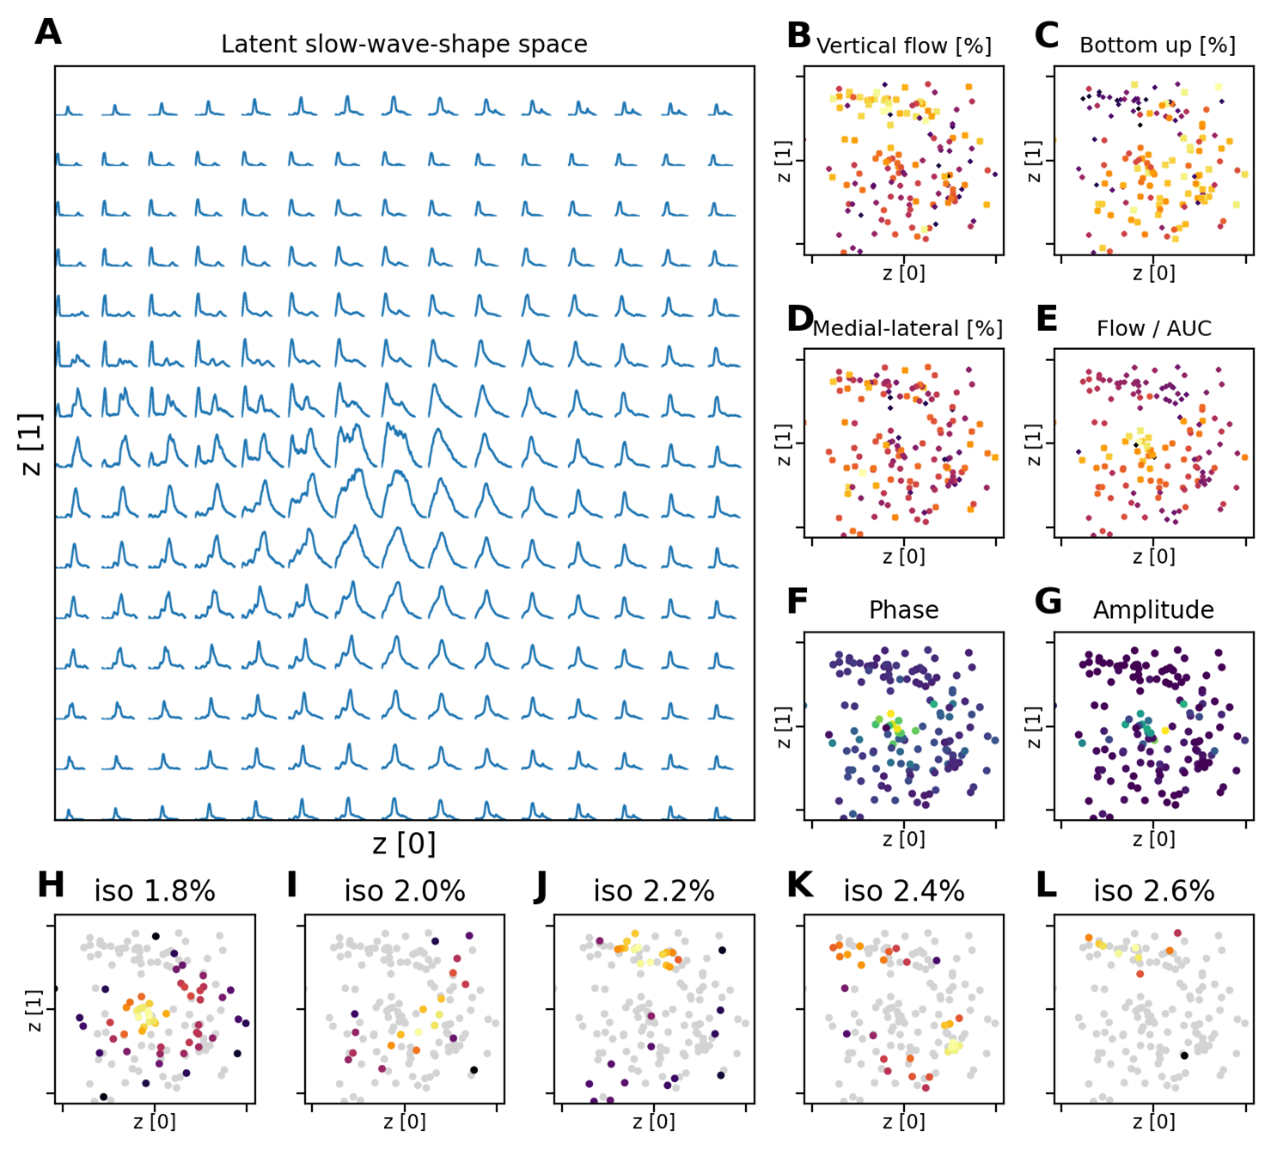
\includegraphics[width=\textwidth,height=\textheight,keepaspectratio]{Figures/slow_wave_shape_space}
\decoRule
\caption[Latent slow wave shape space]{Latent slow wave shape space.\\Note that events with peak-amplitude below 5\% signal change and a high correlation with the hemodynamic breathing signal (r>.3) were excluded from the analysis. Panel A: Latent slow wave shape space. The panel shows a manifold of decodings for different combinations of the activation of the latent-layer neurons z[0] and z[1]. Note that the latent-layer activations are chosen from an evenly spaced grid. The minimal and maximal values for each dimension of this grid are chosen as $\bar{z}\pm\delta\left(z\right)$ with z = encoder(x). The decodings of the vectors are scaled according to the predictions of the width and height and plotted using a square root scale to ensure good visibility of small magnitude events. Panel B: The proportion of the absolute vertical flow as a fraction of the absolute flow during each wave. Panel C: The proportion of bottom-up flow as a fraction of the vertical flow. Panel D: The fraction of medial-lateral flow as a fraction of horizontal flow. Panel E: The ratio between mean absolute flow and the area under the curve of the mean percentage change for each wave. Panel F: The phase/duration of each event. Panel G: The distribution of the amplitude (peak of mean percentage change) for each of the events. Panels H-L: The distribution of samples in latent slow wave shape space.}
\label{fig:slow_wave_shape_space}
\end{figure}


\begin{figure}[!htb]
\centering
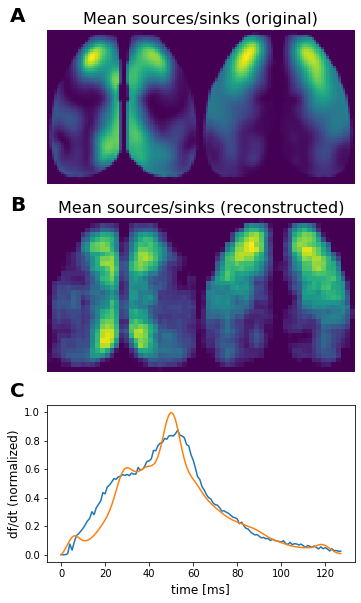
\includegraphics[width=\textwidth,height=\textheight,keepaspectratio]{Figures/reconstructions_example_mixed_input}
\decoRule
\caption[Examples for reconstructions of the mixed input model]{Examples for reconstructions of the mixed input model.// Panel A: The distribution of sources (left) and sinks (right). Panel B: The reconstructions of image shown in Panel A. Panel C: The respective df/f signal and the reconstructed signal.}
\label{fig:reconstructions_example_mixed_input}
\end{figure}

\begin{figure}[!htb]
\centering
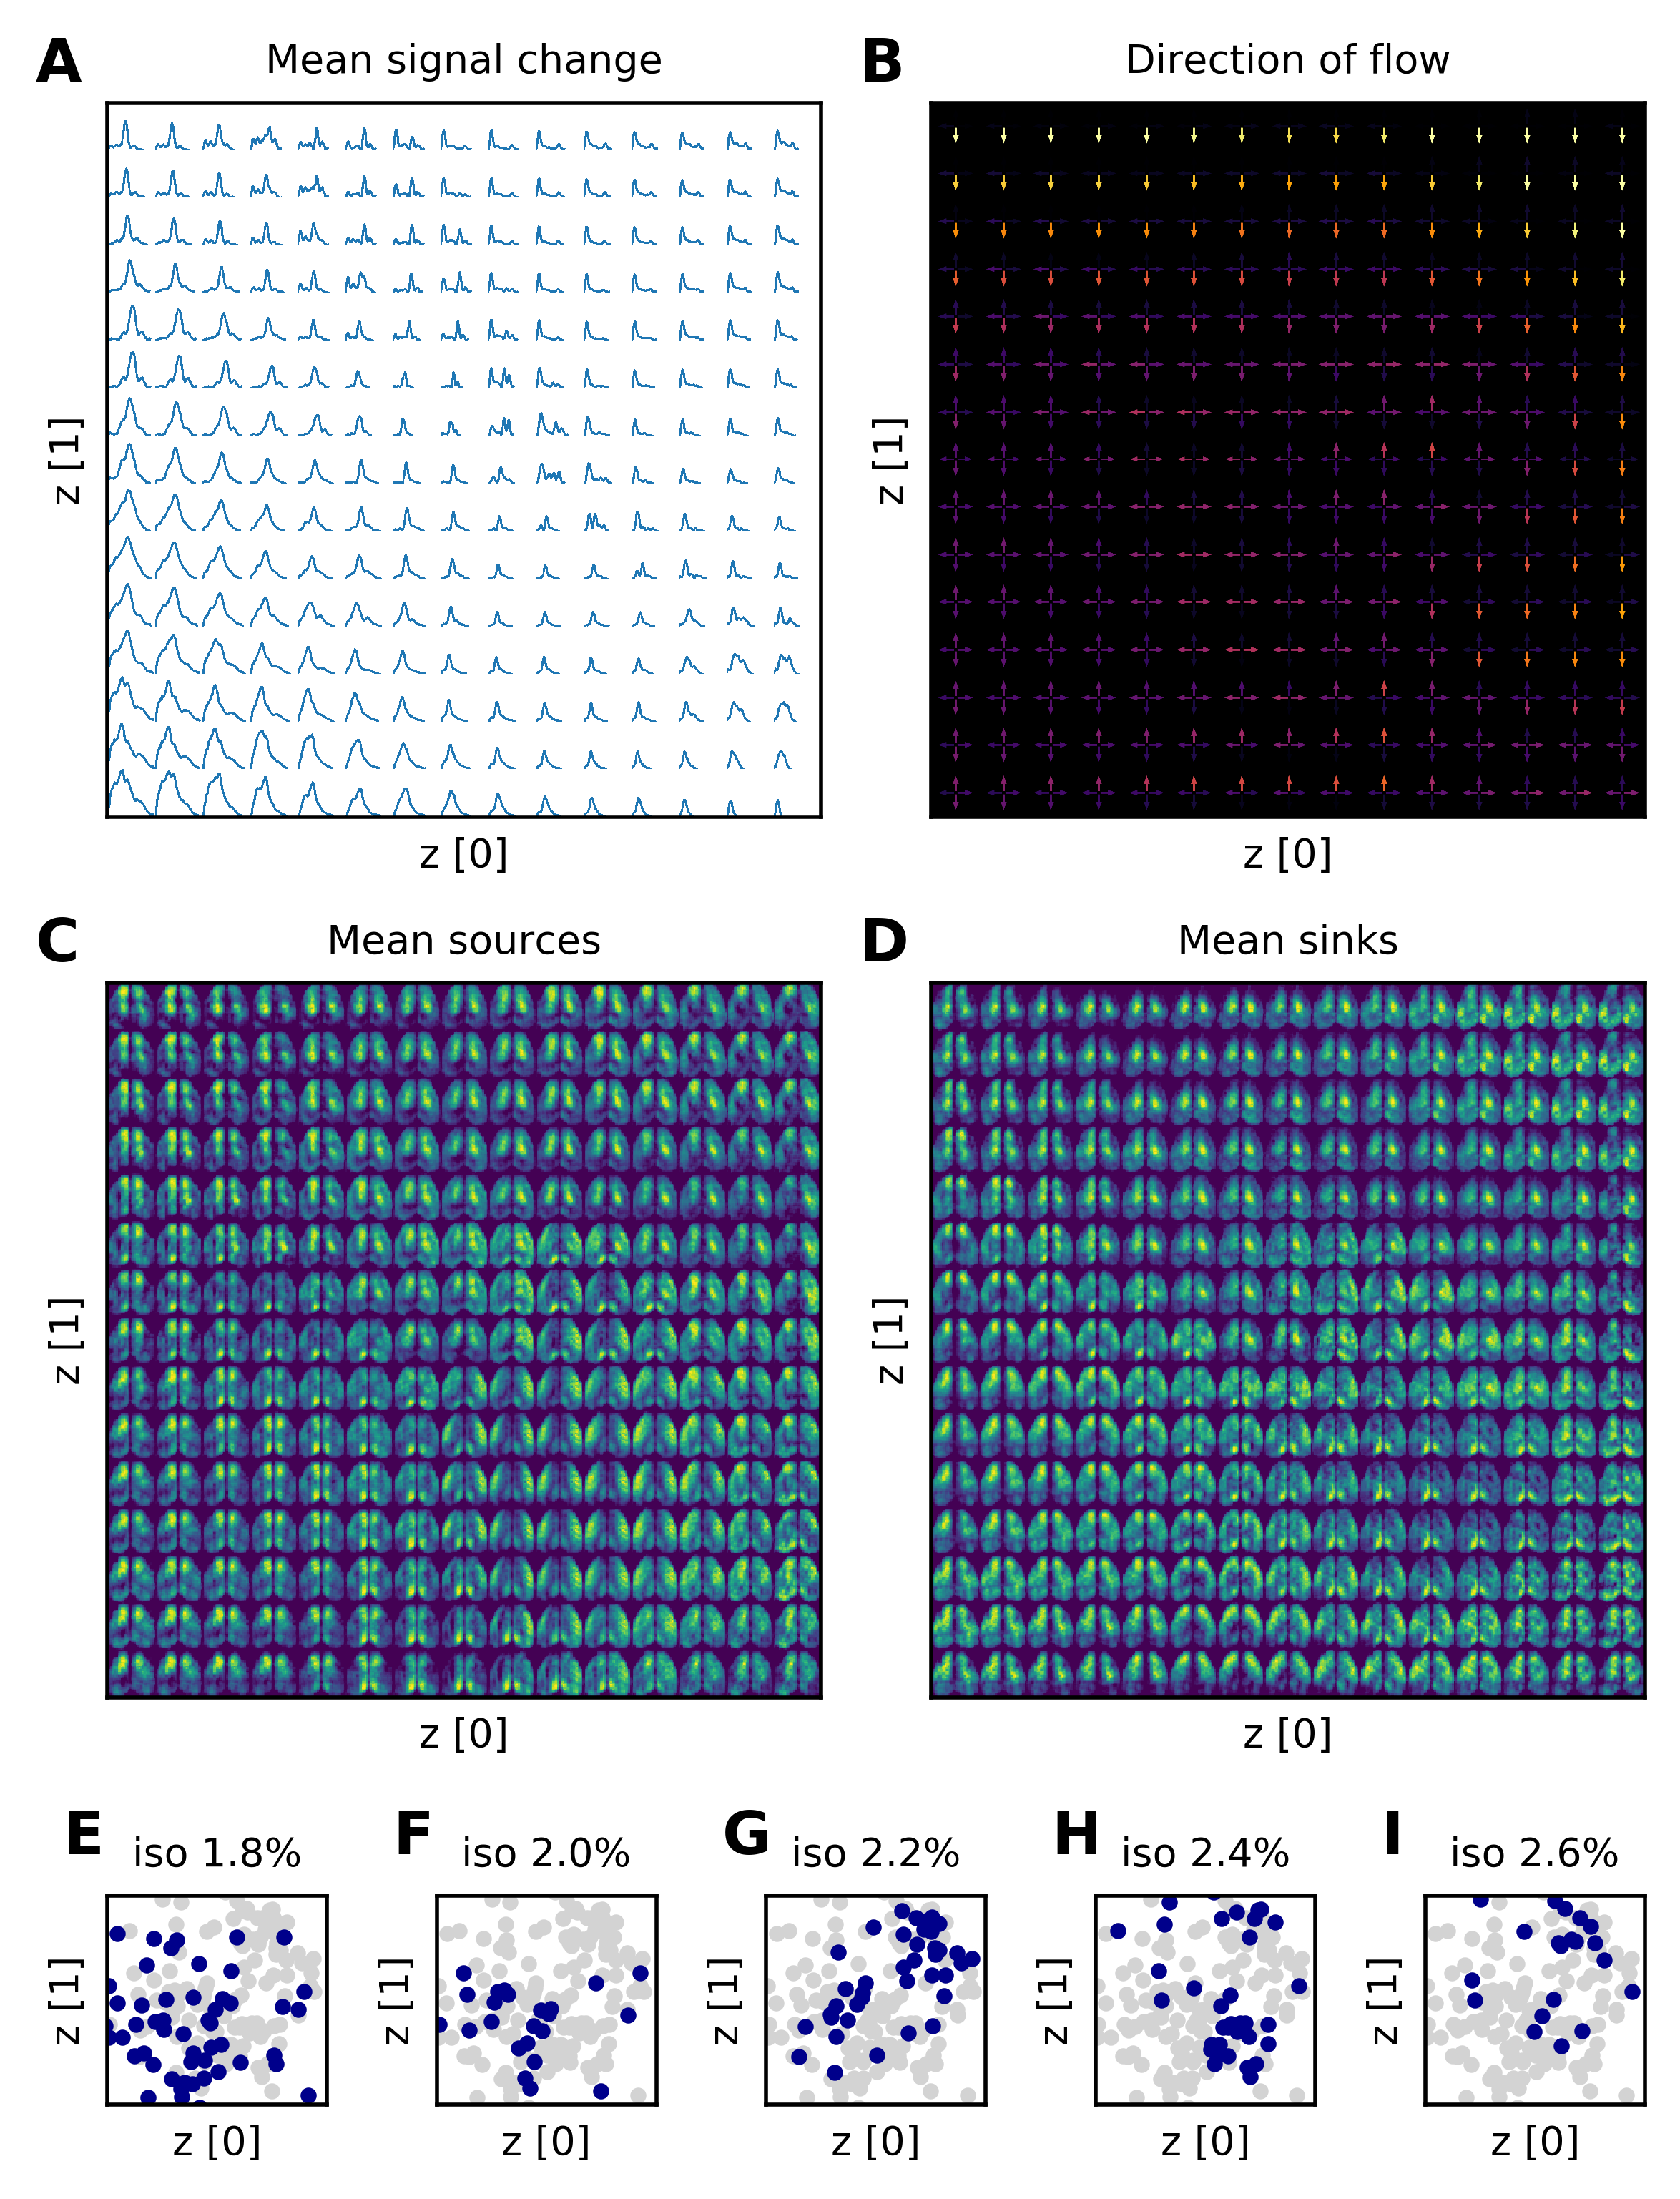
\includegraphics[width=\textwidth,height=\textheight,keepaspectratio]{Figures/latent_slow_wave_space}
\decoRule
\caption[Latent slow wave space]{Latent slow wave space\\The depiction shows the results of for the mixed input model. Note that events with peak-amplitude below 5\% signal change and a high correlation with the hemodynamic breathing signal (r>.3) were excluded from the analysis. Panel A: Slow wave shape space. The panel shows the reconstructions of the df/f signal for the mixed input model. Duration and amplitude are square root scaled. The subspace covered for all reconstruction manifolds is $\bar{z}\pm\delta\left(z\right)$ with z = encoder(x). Panel B: The direction of flow. Arrows indicate the reconstructions for the ratio of flow for each event. Note that upwards flow dominates in the lower center, flow occurs in all directions rather evenly in the middle left portion while downwards flow dominates for events in the upper right area. Panel C and D: The reconstructions of the sources and sinks. Note that differences in the distibution of sources and sinks are most strongly pronounced in the lower central part. Panel E-I: The distribution of samples of different experimental conditions in latent slow wave space. Note that the density of the distribution for overlapping points is color-coded. All samples that do not belong to the respective condition are plotted in grey.}
\label{fig:latent_slow_wave_space}
\end{figure}

\begin{figure}[!htb]
\centering
\includegraphics[width=\textwidth,height=\textheight,keepaspectratio]{Figures/latent_flow_space}
\decoRule
\caption[Latent slow wave flow space]{Latent slow wave flow space\\ The depiction illustrates the relationship between the signal change of the flouroscence signal (df/f) and periods of upwards and downwards flow. Autoencoder 3 was used to compute the mappings to latent space and decodings using an evenly spaced grid that covers the majority of points. Panel A: A reconstruction manifold where blue lines relate to the df/f signal. Green lines indicate the strength of upwards flow, as measured by the mean Y component per frame, for periods where this measure is positive. Analogously orange relates to downwards flow. Note that the periods where the vertical flow is most pronounced coincide with the rising phase of the df/f signal. For some events several peaks in flow occur that correspond to several oscillations in the df/f signal. Moreover the preferred direction of flow is not necessarily the same during these subsegements. Panel B-F: The distribution of samples of different experimental conditions in latent slow wave flow space. Note that the density of the distribution for overlapping points is color-coded. All samples that do not belong to the respective condition are plotted in grey.}
\label{fig:latent_flow_space}
\end{figure}

Nunc posuere quam at lectus tristique eu ultrices augue venenatis. Vestibulum ante ipsum primis in faucibus orci luctus et ultrices posuere cubilia Curae; Aliquam erat volutpat. Vivamus sodales tortor eget quam adipiscing in vulputate ante ullamcorper. Sed eros ante, lacinia et sollicitudin et, aliquam sit amet augue. In hac habitasse platea dictumst.

%-----------------------------------
%	SUBSECTION 2
%-----------------------------------
